\documentclass[crop,tikz]{standalone}% 'crop' is the default for v1.0, before it was 'preview'
\usetikzlibrary{calc,positioning,shapes.geometric,backgrounds,fit,shadows.blur,arrows.meta}
\begin{document}
    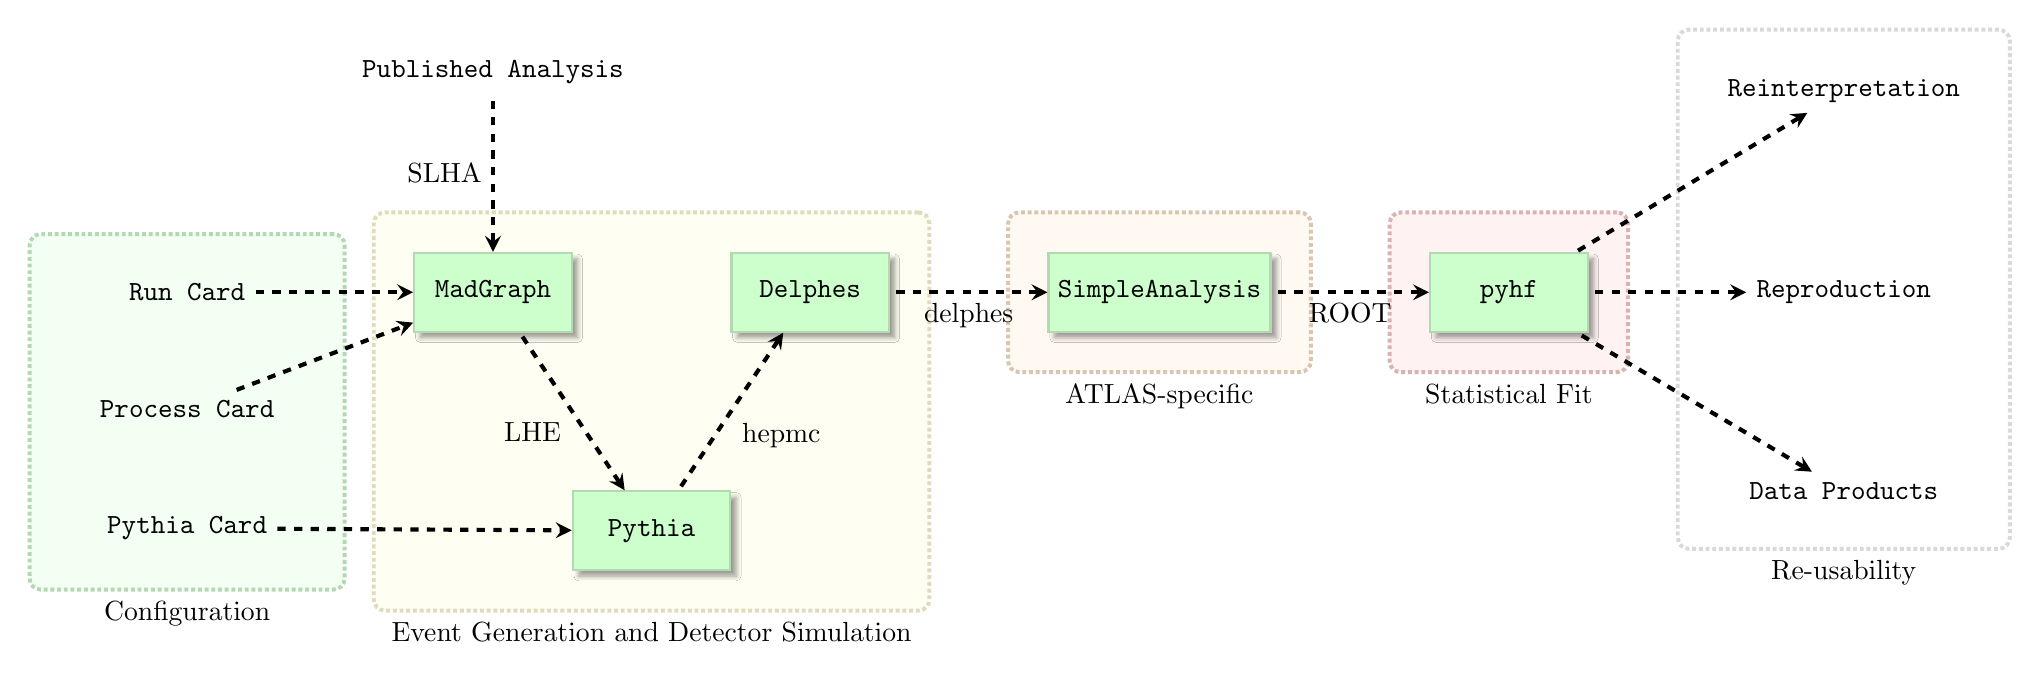
\begin{tikzpicture}[
      align=center,
      >=stealth,
      node distance=4cm,
      auto,
      line width=0.3mm,
      colorit/.style={
        draw=#1!50!black!30,
        fill=#1!20,
        thick,
        blur shadow={shadow blur steps=5}
      },
      colorit/.default=black,
      tool/.style={rectangle,colorit=green, minimum height=1cm, minimum width=2cm},
      boxit/.style={
        draw=#1!50!black!30,
        fill=#1!5,
        densely dotted,
        line width=0.5mm,
        rounded corners
      },
      boxit/.default=yellow
    ]

      \node (start) at (0,0) {\texttt{Published Analysis}};
      \node[tool, below=2cm of start] (madgraph) {\texttt{MadGraph}}
        edge [<-, line width=1.5pt, dashed] node[auto, align=center] {SLHA} (start);
      \node[tool, below right=2cm and 1cm of madgraph, anchor=north] (pythia) {\texttt{Pythia}}
        edge [<-, line width=1.5pt, dashed] node[auto] {LHE} (madgraph);
      \node[tool, right=2cm of madgraph] (delphes) {\texttt{Delphes}}
        edge [<-, line width=1.5pt, dashed] node[auto] {hepmc} (pythia);
      \node[tool, right=2cm of delphes] (simpleanalysis) {\texttt{SimpleAnalysis}}
        edge [<-, line width=1.5pt, dashed] node[auto] {delphes} (delphes);
      \node[tool, right=2cm of simpleanalysis] (pyhf) {\texttt{pyhf}}
        edge [<-, line width=1.5pt, dashed] node[auto] {ROOT} (simpleanalysis);
      \node[right=2cm of pyhf] (reproduction) {\texttt{Reproduction}}
        edge [<-, line width=1.5pt, dashed] node[auto] {} (pyhf);
      \node[above=2cm of reproduction] (reinterpretation) {\texttt{Reinterpretation}}
        edge [<-, line width=1.5pt, dashed] node[auto] {} (pyhf);
      \node[below=2cm of reproduction] (products) {\texttt{Data Products}}
        edge [<-, line width=1.5pt, dashed] node[auto] {} (pyhf);

      \node[left=2cm of madgraph] (runcard) {\texttt{Run Card}}
        edge [->, line width=1.5pt, dashed] node[auto] {} (madgraph);
      \node[below=1cm of runcard, anchor=north] (proccard) {\texttt{Process Card}}
        edge [->, line width=1.5pt, dashed] node[auto] {} (madgraph);
      \node[below=1cm of proccard, anchor=north] (pythiacard) {\texttt{Pythia Card}}
        edge [->, line width=1.5pt, dashed] node[auto] {} (pythia);

      \begin{scope}[on background layer]
        \node [label={below:Configuration}, minimum width=4cm, inner sep=0.5cm, boxit=green, fit=(runcard) (proccard) (pythiacard)] {};
        \node [label={below:Event Generation and Detector Simulation}, inner sep=0.5cm, boxit, fit=(madgraph) (pythia) (delphes)] {};
        \node [label={below:ATLAS-specific}, inner sep=0.5cm, boxit=orange, fit=(simpleanalysis)] {};
        \node [label={below:Statistical Fit}, inner sep=0.5cm, boxit=red, fit=(pyhf)] {};
        \node [label={below:Re-usability}, inner sep=0.5cm, boxit=white, fit=(reproduction) (reinterpretation) (products)] {};
      \end{scope}
    \end{tikzpicture}
\end{document}
